\documentclass[compress]{beamer}
\usetheme{Warsaw}
\usecolortheme{seagull}
\setbeamertemplate{headline}{}
\beamertemplatenavigationsymbolsempty
\useoutertheme{infolines}

\usepackage{biblatex}
\bibliography{bibliography}
\renewcommand{\footnotesize}{\tiny}

\setbeamersize{text margin left=10pt,text margin right=10pt}
\setbeamertemplate{enumerate items}[default]
\setbeamertemplate{itemize items}[default]

%\addtobeamertemplate{navigation symbols}{}{%
%    \usebeamerfont{footline}%
%    \usebeamercolor[fg]{footline}%
%    \hspace{1em}%
%    \insertframenumber/\inserttotalframenumber
%}

\usepackage{graphicx}
\graphicspath{{/Users/jlochman/Desktop/Diploma-thesis/Chapter3/}}
\usepackage{epstopdf}
\usepackage{booktabs} 
\usepackage{courier}
\usepackage{color}
\usepackage{tikz}

\setbeamercovered{transparent}

\PassOptionsToPackage{demo}{graphicx}
\def\Put(#1,#2)#3{\leavevmode\makebox(0,0){\put(#1,#2){#3}}}

\newcommand{\GeV}{\,\text{GeV}}
\newcommand{\TeV}{\,\text{TeV}}
\newcommand{\pt}{p_{T}}

\title[High $\pt$ jets]{Jety s vysokou p\v{r}\'{i}\v{c}nou hybnost\'{i} v RunII
experimentu ATLAS} 
\author{Jan Lochman}
\institute[FNSPE CTU] 
{
  FJFI \v{C}VUT \\
  \medskip
  \medskip
  \large
  Obhajoba diplomov\'{e} pr\'{a}ce \\ 
  \medskip
}
\date{\today}

\begin{document}

%------------------------------------------------

\begin{frame}
\titlepage 
\end{frame}

\section{Introduction}

\begin{frame}
\frametitle{\'{U}vod}
\begin{block}{C\'{i}l pr\'{a}ce}
  C\'{i}lem diplomov\'{e} pr\'{a}ce bylo p\v{r}ipravit anal\'{y}zu
  inkluzivn\'{i}ho
  \'{u}\v{c}inn\'{e}ho pr\r{u}\v{r}ezu
  produkce jet\r{u} a porovnat data s p\v{r}edpov\v{e}d\'{i} next-to-leading order
  QCD v r\'{a}mci
  Standard Model skupiny experimentu ATLAS pro pou\v{z}it\'{i} po
  spu\v{s}t\v{e}n\'{i} urychlova\v{c}e s
  t\v{e}\v{z}i\v{s}\v{t}ovou energi\'{i} 13 TeV.
\end{block}
\begin{block}{Osnova prezentace}
\begin{itemize}
  \item \textbf{\'{U}vod} 

    Jet, Inkluzivn\'{i} jet, K \v{c}emu?
  \item \textbf{Anal\'{y}za dat}

    Charakteristika dat, Rekonstrukce jet\r{u}, Unfolding.
  \item \textbf{Porovn\'{a}n\'{i} dat s p\v{r}edpov\v{e}d\'{i} NLO QCD}

    Neur\v{c}itosti v p\v{r}edpov\v{e}d\'{i}ch QCD, LO vs. NLO QCD.

  \item \textbf{Z\'{a}v\v{e}r}
\end{itemize}
\end{block}
\end{frame}
%------------------------------------------------

\begin{frame}
\frametitle{Why Do We Need Jets?}
\onslide<1->
\begin{columns}[onlytextwidth]
  \begin{column}{0.5\textwidth}
    \textbf{Gluon radiation cross section:}
    \textbf{Divergences:}
    \begin{itemize}
      \item \textit{\color{red}Infrared} ($E_k = 0$)
      \item \textit{\color{red}Collinear} ($\theta = 0$)
    \end{itemize}
    \textbf{Jet:} A group of collimated particles
  \end{column}
  \begin{column}{0.5\textwidth}
    \begin{equation*}
      \sigma_{q \rightarrow qg} \sim \frac{d\theta}{|\sin\theta|}
      \frac{dE_k}{E_k}
    \end{equation*}
    \begin{figure}[b]
      \centering
      
\includegraphics[width=\textwidth]{{../PrezentationATLASmeeting/gluonRadiation}.png}
    \end{figure}
  \end{column}
\end{columns}
\onslide<2->
\textbf{Jet algorithm:} A prescription, how particles (or other objects) are clustered
  into separate jets. It should fulfill
\begin{columns}[onlytextwidth]
  \begin{column}{0.7\textwidth}
      \begin{itemize}
        \item \textit{Infrared safety:} The presence of an additional soft particle
          should not affect the recombination of particles into a jet.
        \item \textit{Collinear safety:} Jet reconstruction should not depend on the
          fact, if the energy is carried by one particle, of if the particle is
          split into more collinear particles.
      \end{itemize}
  \end{column}
  \begin{column}{0.3\textwidth}
    \begin{figure}[b]
      \centering
      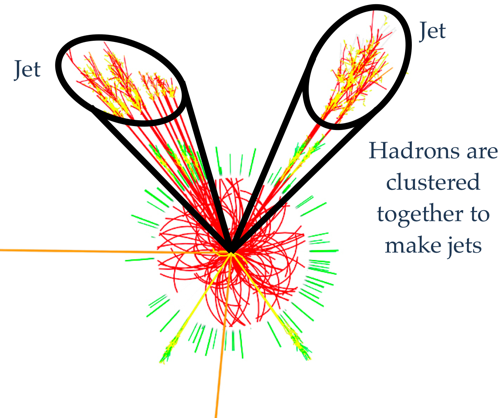
\includegraphics[width=\textwidth]{{../PrezentationATLASmeeting/clustering}.png}
    \end{figure}
  \end{column}
\end{columns}
$q$ or $g$ {\color{red}CANNOT} be observed. Jets {\color{red}CAN}.
\end{frame}



\begin{frame}
\frametitle{Inclusive Jets} 
\scriptsize
Inclusive jet double differential cross section in $\pt$ and rapidity
$y$ (inclusive means $pp~\rightarrow$~jet~+~''anything'') in Run~II of the ATLAS
Experiment ($\sqrt{s}=13\TeV$).
2013 Analysis {\footfullcite{Analysis2012}}:
\begin{columns}[onlytextwidth]
  \begin{column}{0.5\textwidth}
    \begin{figure}[b]
      \centering
      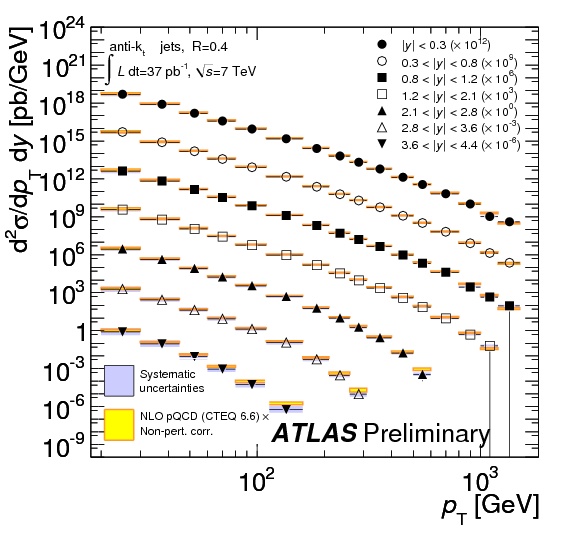
\includegraphics[width=\textwidth]{{../PrezentationATLASmeeting/ATLASinclusive04}.png}
    \end{figure}
  \end{column}
  \begin{column}{0.5\textwidth}
    \begin{block}{Why Inclusive Jets?}
      \begin{itemize}
        \item They Cover a \textit{\color{red}wide range of momentum transfers}
          ($\sim 1 \GeV - 1 \TeV$ on the LHC) $\rightarrow$ predictions sensitive to
          the properties of the running coupling constant $\alpha_S$
        \item They probe the structure of proton at \textit{\color{red}small
        distance scales}
        \begin{equation*}
          \lambda \sim 1/\pt \sim \TeV^{-1} \sim 10^{-19}\,\text{m}
        \end{equation*}
        \item They contribute to our understanding of PDFs
        \item They \textit{\color{red}appreciate the increase in the center-of-mass
        energy} as no other physics process observed on hadron colliders
      \end{itemize}
    \end{block}
  \end{column}
\end{columns}
\end{frame}


\section{Data Analysis}
\subsection{Data Characteristics}

\begin{frame}
\frametitle{Jet Reconstruction}
Jet can be defined on a \textit{three different levels of collision}:
\begin{itemize}
  \item \textbf{Parton level} - quarks, gluons and other particles created just after the
    collision. Directly connected to the QCD processes.
  \item \textbf{Particle level} - particles created by the hadronization. 
  \item \textbf{Detector level} - recorded signal. Detector imperfections cause a
    \textit{\color{red}distortion of observables}.
\end{itemize}
\begin{figure}[b]
  \centering
  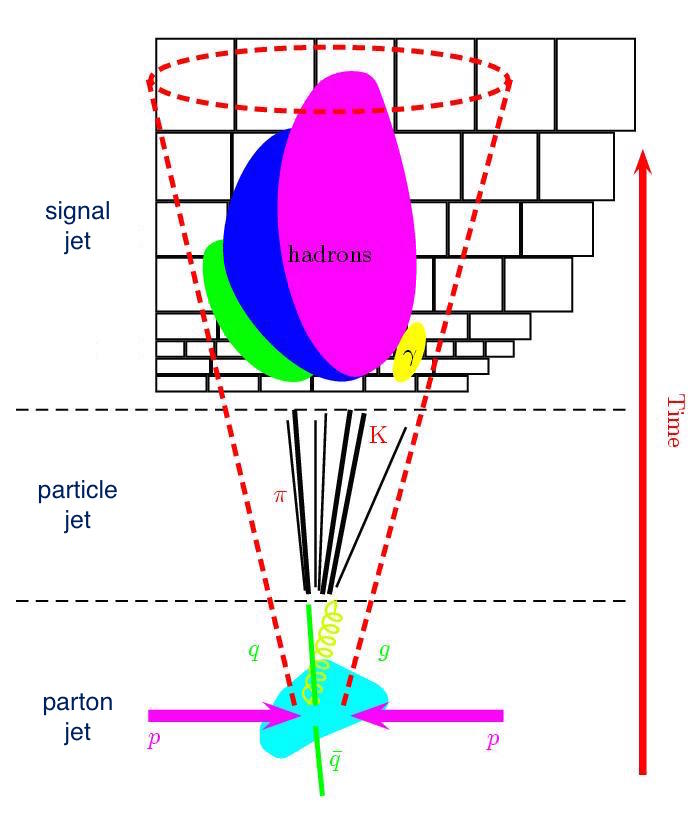
\includegraphics[width=0.7\textwidth]{{../Chapter2/JetPhases}.png}
\end{figure}
\end{frame}

\begin{frame}
\frametitle{Data Characteristics}
\begin{columns}[onlytextwidth]
  \begin{column}{0.4\textwidth}
\begin{itemize}
  \item $pp$ collisions at $\sqrt{s}=13\TeV$, anti-$k_t$ jet algorithm with
    $R=0.4$, CT10 PDFs, AU2
  \item Measuring of inclusive jet double differential cross section in $\pt$
    and rapidity $y$ 
\end{itemize}
  \end{column}
  \begin{column}{0.6\textwidth}
\begin{figure}[b]
  \centering
  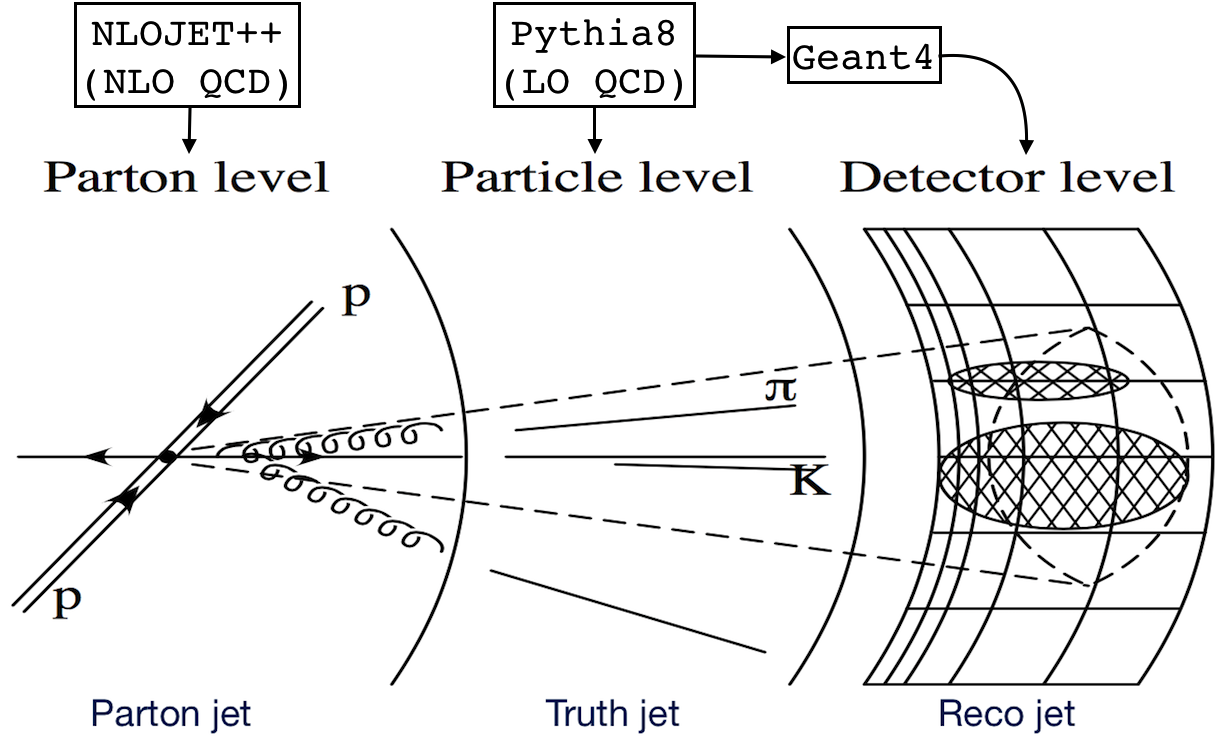
\includegraphics[width=\textwidth]{{../PrezentationATLASmeeting/DataChar}.png}
\end{figure}
  \end{column}
\end{columns}
\begin{itemize}
  \item \textbf{Parton level} - cross section prediction calculated with NLOJET++ program
    (\textit{\color{red}NLO~QCD}).  
  \item \textbf{Particle level} - events generated by \textsc{Pythia8}
    (\textit{\color{red}LO~QCD}).  
  \item \textbf{Detector level} -
    detector response on \textsc{Pythia8} events obtained
    by \textsc{Geant4} full detector simulation. 
\end{itemize} 
\textbf{Jet Matching} - for each truth jet, corresponding reco jet is found. 
\end{frame}

\subsection{Jet Corrections}

\begin{frame}
\frametitle{Jet Corrections}
\begin{itemize}
  \item Correct observables derived from detector to particle level by
    removing the detector effects
  \item Two main procedures - \textit{\color{red}Calibration} and
    \textit{\color{red}Unfolding}
\end{itemize}
\begin{figure}[b]
  \centering
  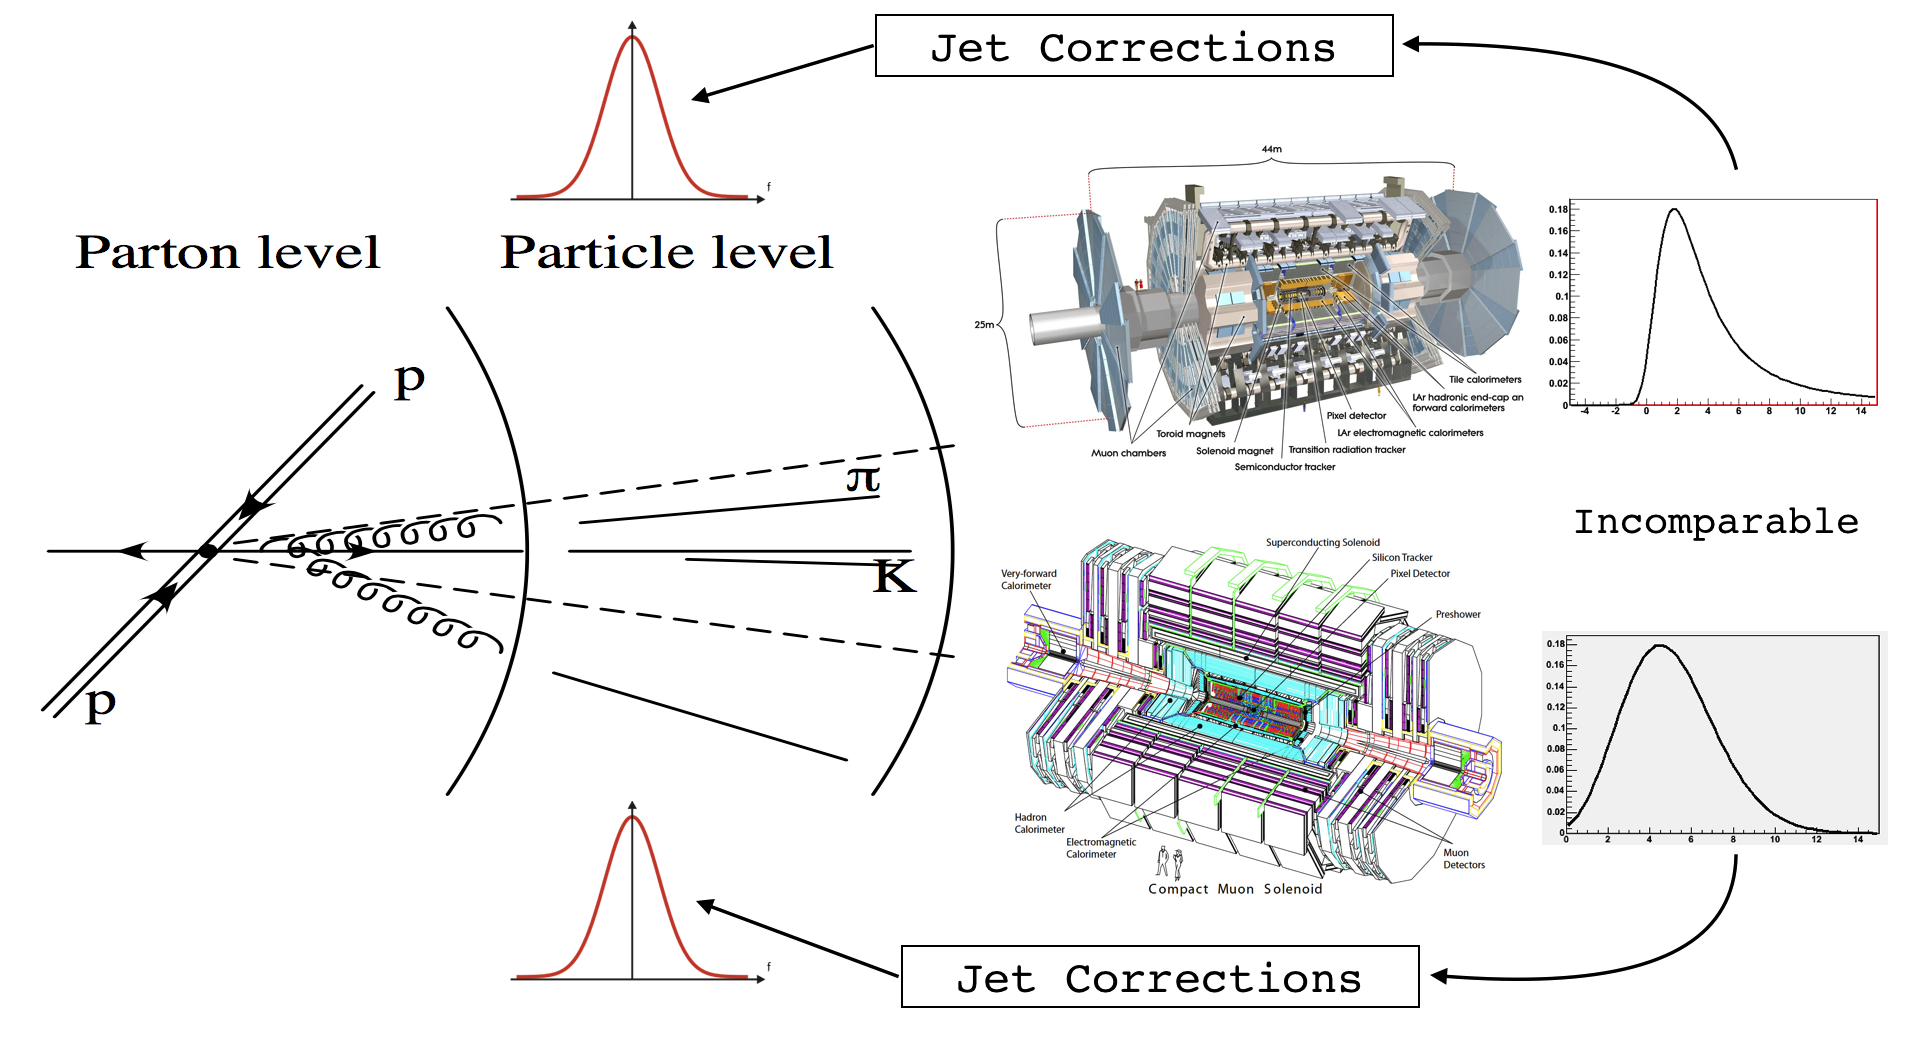
\includegraphics[width=0.9\textwidth]{{../PrezentationATLASmeeting/JetCorrections}.png}
\end{figure}
\end{frame}

\subsection{Unfolding}

\begin{frame}
\frametitle{Unfolding}
\begin{itemize}
  \item Final step of jet corrections.
  \item Tries to minimize the effects of detector \textit{\color{red}finite resolution}.
  \item \textit{\color{red}Analysis dependent}.
\end{itemize}
\begin{figure}[b]
  \centering
  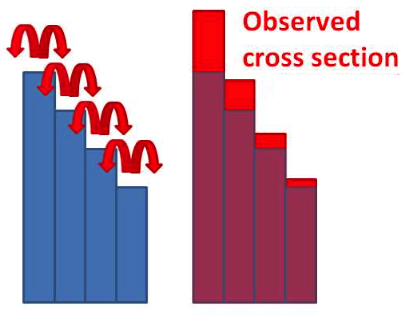
\includegraphics[width=0.39\textwidth]{{../PrezentationATLASmeeting/UnfoldingEffect}.png}
  \includegraphics[width=0.6\textwidth]{{SignalVSTruth}.eps}
\end{figure}
\end{frame}

\begin{frame}
\frametitle{Unfolding - Mathematical Formulation}
\begin{itemize}
  \onslide<1-> \item \textbf{I want:} $f(\pt)$ (distribution of inclusive jet $\pt$ for $\pt \in
    \langle a, b \rangle$)
  \item From detector, \textbf{I get:} $g(x)$ (distribution of unphysical variable
    $x$)
  \begin{equation*}
    g(x) = \int_a^b A(x,\pt) f(\pt) d\pt
  \end{equation*}
  \item Detector smearing described by $A(x,\pt)$
  \item Complicated \textit{\color{red}integral~equation} for $f(\pt)$
  \onslide<2-> \item Luckily $g(x)$ and $f(\pt)$ are for practical purpose discretized and in
    analysis, I assume $x \in \langle a, b \rangle$, $N(i) \subset \langle
    a , b \rangle$ 
  \begin{equation*}
    g_i = \int_{N(i)}g(x)dx \quad , \quad f_i = \int_{N(i)}f(\pt)d\pt
  \end{equation*}
  \item So the response of the detector is described by a ''simple''
    \textit{\color{red}matrix~equation}, with $A$ being called
    \textit{\color{red}Transfer Matrix} 
  \begin{equation*}
    g = A f
  \end{equation*}
\end{itemize}
\end{frame}


\subsection{Unfolding}

\begin{frame}
\frametitle{Inputs for Unfolding}
Unfolding(calibrated reco spectrum) $\approx$ truth spectrum
\begin{itemize}
  \item Inputs for unfolding procedure 
    \begin{itemize}
      \item \textbf{Matching efficiencies} - describing the ratio of matched jets to all jets
      \item \textbf{Transfer matrix} $A_{ij}$ - containing the number of reco jets in bin $i$ with
        a matched truth jets generated in bin $j$
    \end{itemize}
  \item I test {\color{red}two approaches} to the unfolding, allowing a dealing with the
    double binning (in $\pt$ and $y$)
\end{itemize}
\begin{enumerate}
  \item \textbf{Simple unfolding}
    \\
    Matching jets within different rapidity bins is not allowed. There are
    {\color{red}8~independent} 46x46 transfer matrices, one for each rapidity
    bin (46~=~number of $\pt$ bins)
  \item \textbf{2D unfolding}
    \\
    Matching within different rapidity bins allowed. {\color{red}Only one} 368x368 transfer
    matrix ($368=8 \times 48$)
\end{enumerate}
\end{frame}

\begin{frame}
\frametitle{Transfer Matrices}
\begin{columns}[onlytextwidth]
  \begin{column}{0.5\textwidth}
    \begin{figure}[H]
      \centering
    Simple unfolding
      \includegraphics[width=\textwidth]{{unfold_matrix_firstBin}.eps}
    \end{figure}
  \end{column}
  \begin{column}{0.5\textwidth}
    \begin{figure}[H]
      \centering
    2D unfolding
      \includegraphics[width=\textwidth]{{unfold_matrix_all}.eps}
    \end{figure}
  \end{column}
\end{columns}
\end{frame}

\begin{frame}
\frametitle{Unfolding Results}
\begin{columns}[onlytextwidth]
  \begin{column}{0.5\textwidth}
    \begin{figure}[H]
      \centering
    Reco and Unfolded vs. Truth Spectrum
      \includegraphics[width=\textwidth]{{SignalUnfolded_VS_Truth0Compare}.eps}
    \end{figure}
  \end{column}
  \begin{column}{0.5\textwidth}
    \begin{figure}[H]
      \centering
    Simple and 2D unfolded vs. Truth Spectrum
      \includegraphics[width=\textwidth]{{UnfoldedSimpleComplex_VS_Truth0Compare}.eps}
    \end{figure}
  \end{column}
\end{columns}
\end{frame}

\section{NLO QCD Predictions}
\subsection{Introduction}

\begin{frame}
\frametitle{NLO QCD Prediction}
\begin{itemize}
  \item NLO QCD predictions on parton level for $\sqrt{s}=8\TeV$ and
    $\sqrt{s}=13\TeV$
  \onslide<1-> \item \textit{\color{red}Theoretical uncertainties} which are taken into account
  \begin{itemize}
    \item \textbf{Scale uncertainty}

      Choice of renormalization and factorization scales, including
      neglecting the higher order terms beyond the NLO
    \item \textbf{$\alpha_S$ uncertainty}

      Because of experimental measurements of $\alpha_S$.
    \item \textbf{PDF uncertainty}

      Prediction depends on the concrete choice of a PDF
  \end{itemize}
  \onslide<2-> \item \textit{\color{red}Other corrections} (not so significant
    \footfullcite{Analysis2012})
  \begin{itemize}
    \item \textbf{Nonperturbative corrections}

      Hadronization and Underlying Event corrections.
    \item \textbf{Electroweak corrections}

      Next to the QCD processes, the electroweak processes should be assumed.
  \end{itemize}
\end{itemize}
\end{frame}

\subsection{Prediction Properties}

\begin{frame}
\frametitle{NLO Systematic Errors}
\begin{columns}[onlytextwidth]
  \begin{column}{0.5\textwidth}
    \begin{figure}[H]
      \centering
      $\sqrt{s}=8\TeV$
      \includegraphics[width=\textwidth]{{NLO_Systematics8_TeV0}.eps}
    \end{figure}
  \end{column}
  \begin{column}{0.5\textwidth}
    \begin{figure}[H]
      \centering
      $\sqrt{s}=13\TeV$
      \includegraphics[width=\textwidth]{{NLO_Systematics13_TeV0}.eps}
    \end{figure}
  \end{column}
\end{columns}
\end{frame}

\begin{frame}
\frametitle{Comparison of NLO QCD Predictions}
\begin{figure}[b]
  \centering
  \includegraphics[width=\textwidth]{{PredictionCompare0}.eps}
\end{figure}
\end{frame}

\subsection{Comparison with LO}

\begin{frame}
\frametitle{Comparison of LO and NLO QCD}
\begin{figure}[b]
  \centering
  \includegraphics[width=0.7\textwidth]{{Truth_VS_Prediction0Compare}.eps}
\end{figure}
\end{frame}

\section{Conclusion}

\begin{frame}
\frametitle{Thesis Conclusions}
\begin{block}{Unfolding}
  Two approaches were probed.
  
  No significant differences between these two approaches imply, for the real
  analysis, the {\color{red}Simple Unfolding approach should be used} for its simpler
  implementation.

  Agreement of the unfolded $\pt$ spectra with the truth $\pt$ spectra up to
  systematic error $<10^{-3}\,\%$.
\end{block}
\begin{block}{LO and NLO QCD}
  {\color{red}Significant differences} showing the influence of the NLO QCD
  processes on physical observables.
\end{block}
\end{frame}

\end{document} 
